%%%%%%%%%%%%%%%%%%%%%%%%%%%%%%%%%%%%%%%%%
% Short Sectioned Assignment LaTeX Template Version 1.0 (5/5/12)
% This template has been downloaded from: http://www.LaTeXTemplates.com
% Original author:  Frits Wenneker (http://www.howtotex.com)
% License: CC BY-NC-SA 3.0 (http://creativecommons.org/licenses/by-nc-sa/3.0/)
%%%%%%%%%%%%%%%%%%%%%%%%%%%%%%%%%%%%%%%%%

%----------------------------------------------------------------------------------------
%   PACKAGES AND OTHER DOCUMENT CONFIGURATIONS
%----------------------------------------------------------------------------------------

\documentclass[10pt,a4paper,spanish]{article}

% ---- Entrada y salida de texto -----

\usepackage[spanish]{babel} 
\usepackage[T1]{fontenc} % Use 8-bit encoding that has 256 glyphs
\usepackage[utf8]{inputenc}
\usepackage{cite}
% \usepackage{spreadtab}
% \usepackage{fourier} % Use the Adobe Utopia font for the document - comment this line to return to the LaTeX default
\usepackage[usenames, dvipsnames]{color}
\usepackage[table]{xcolor}
\usepackage{colortbl}
\usepackage[bookmarks=true,colorlinks=true,linkcolor=red,citecolor=blue]{hyperref}
% \usepackage{cite}
% \usepackage[official]{eurosym}
\usepackage{tikz}
% \usepackage{pgfplots}
% \pgfplotsset{compat=1.5}
\usepackage{minted}

\usepackage{subfigure}

% \usepackage{pseudocode}

% ---- Otros paquetes ----
\usepackage{enumerate}
\usepackage{amsmath,amsfonts,amsthm,amssymb} % Math packages
\usepackage{graphics,graphicx} %para incluir imágenes y notas en las imágenes
% Para hacer tablas comlejas
%\usepackage{multirow}
%\usepackage{threeparttable}

\usepackage[a4paper, margin=1.3in]{geometry}


\usepackage{sectsty} % Allows customizing section commands
\allsectionsfont{\centering \normalfont\bfseries\scshape} % Make all sections centered, the default font and small caps
\usepackage{fancyhdr}
\pagestyle{fancy}
%con esto nos aseguramos de que las cabeceras de capítulo y de sección vayan en minúsculas

\renewcommand{\sectionmark}[1]{%
      \markright{\thesection\ #1}}
\fancyhf{} %borra cabecera y pie actuales
\fancyhead[LE,RO]{{\bfseries Práctica 4}}
\fancyhead[LO]{\bfseries Marta Gómez}
\fancyfoot[C]{\thepage{}}
\renewcommand{\headrulewidth}{0.5pt}
\renewcommand{\footrulewidth}{0pt}
\addtolength{\headheight}{0.5pt} %espacio para la raya
\fancypagestyle{plain}{%
      \fancyhead{} %elimina cabeceras en páginas "plain"
      \renewcommand{\headrulewidth}{0pt} %así como la raya
}

\numberwithin{equation}{section} % Number equations within sections (i.e. 1.1, 1.2, 2.1, 2.2 instead of 1, 2, 3, 4)
\numberwithin{figure}{section} % Number figures within sections (i.e. 1.1, 1.2, 2.1, 2.2 instead of 1, 2, 3, 4)
\numberwithin{table}{section} % Number tables within sections (i.e. 1.1, 1.2, 2.1, 2.2 instead of 1, 2, 3, 4)

\setlength\parindent{0pt} % Removes all indentation from paragraphs - comment this line for an assignment with lots of text
\setlength{\parskip}{1ex plus 0.5ex minus 0.2ex}

\newcommand{\horrule}[1]{\rule{\linewidth}{#1}} % Create horizontal rule command with 1 argument of height

%----------------------------------------------------------------------------------------
%   TÍTULO Y DATOS DEL ALUMNO
%----------------------------------------------------------------------------------------

\title{
\normalfont \normalsize 
{\bf Redes y Sistemas Complejos} \\ Curso 2016-2017 \\ [25pt] % Your university, school and/or department name(s)
\horrule{0.5pt} \\[0.4cm] % Thin top horizontal rule
\huge \textsc{Práctica 4: \\ Estudio Comparativo de Métodos \\ para Poda y Visualización \\ de Redes } \\ % The assignment title
\horrule{2pt} \\[0.5cm] % Thick bottom horizontal rule
}

\author{\textit{Marta Gómez Macías}} %\\ \texttt{mgmacias95@correo.ugr.es} \\ 75929776Z \\[0.5cm]

% \date{\normalsize\today} % Incluye la fecha actual

% \usepackage{pdflscape}

\newmintedfile[mypy]{python}{
    linenos, % muestra el número de línea
    numbersep=5pt, % separación entre el código y el número de línea
    gobble=0, % columna desde la que empieza a mostrar código
    frame=lines, % dibuja las líneas enmarcando el código
    framesep=2mm, % separación entre la línea y el código
    tabsize=3, % tamaño de la tabulación
}

%----------------------------------------------------------------------------------------
% DOCUMENTO
%----------------------------------------------------------------------------------------

\begin{document}
%Cambiar Cuadros por Tablas y lista de...
\renewcommand{\listtablename}{Índice de tablas}
\renewcommand{\tablename}{Tabla} 

\begin{titlepage}
\begin{center}

\includegraphics[width=0.2\textwidth]{../../ugr}

\normalfont \normalsize 
{\bf Redes y Sistemas Complejos} \\ Curso 2016-2017 \\ [25pt] % Your university, school and/or department name(s)
\horrule{0.5pt} \\[0.4cm] % Thin top horizontal rule
{\huge \textsc{Práctica 4: \\ Caso Práctico de Análisis \\ y Evaluación de \\ Redes}} % The assignment title
\horrule{2pt} \\[0.5cm] % Thick bottom horizontal rule

{\Large \textit{Marta Gómez Macías} \\ \texttt{mgmacias95@correo.ugr.es} \\ 75929776Z \\[0.5cm]

\date{\today}} % Incluye la fecha actual
\end{center}
\end{titlepage}

\tableofcontents % para generar el índice de contenidos

\newpage

% \listoffigures

% \listoftables

\section{Selección del dominio, definición de la pregunta y obtención del conjunto estructural inicial}

\subsection{Selección del dominio y definición de la pregunta}
Llevo muchos años participando activamente en la red social \textit{Twitter}. Durante estos años, he ido siguiendo (y dejando de seguir también) a un montón de gente muy diferente: amigos del instituto, cuentas que ponen tweets interesantes, amigos de la facultad, etc. En mi \textit{Timeline} veo tweets de todo tipo y muy diferentes entre sí, tanto que a veces se me hace algo confuso. Por tanto, me hice la siguiente pregunta: \textbf{¿podría agrupar de una forma sencilla todas las cuentas que sigo por su temática?}

Dándole vueltas a esta pregunta, apliqué la siguiente lógica: los amigos de la facultad que sigo en Twitter, también se siguen entre sí. Al igual que los del instituto o la gente que conocí en un determinado evento. Es decir, si dos de las cuentas que sigo se siguen entre sí, es bastante probable que publiquen Tweets sobre temas muy similares. Así, descubrí que viendo las comunidades que hay entre mis ``amigos'' de Twitter podría agrupar las diferentes cuentas que sigo por temática. Esto se conoce como \textbf{Transitividad}.

\subsection{Obtención del conjunto estructural inicial}
Para obtener los datos, he desarrollado una sencilla aplicación con \textit{Django} y \textit{Tweepy}. He creado una base de datos en \texttt{sqlite3} en la que voy guardando usuarios de Twitter y las personas a las que siguen. Dicha aplicación se encuentra libre en \href{https://github.com/mgmacias95/TwitterFriends}{Github}.

La aplicación, en primer lugar, almacena en la base de datos todas las personas que sigo y, además, todos los usuarios que siguen las personas a las que sigo. Una vez tengo registrados todos mis amigos y los amigos de mis amigos, los relaciono entre sí usando los \texttt{ManyToManyField} de \textit{Django}. Es importante destacar que esta red es \textit{dirigida}, ya que en Twitter un usuario no tiene por qué hacer \textit{follow back}.

Finalmente, como sólo me interesa quedarme con las relaciones entre las personas que yo sigo, hago un filtrado a la hora de exportar la red a formato GDF. Si no hubiese hecho ningún filtrado, trabajaría con una red de 100.000 nodos, que fue los que recopilé en primer lugar.

\section{Construcción de la red compleja a analizar y visualizar}
En mi caso, la red obtenida era bastante pequeña, ya que sólo sigo a unas 540 personas. Por tanto, no he eliminado ningún nodo. Tampoco he eliminado ningún enlace, ya que todos los enlaces tienen el mismo peso y, si elimino algún enlace, pierdo la relación entre dos usuarios. 

Por tanto, debido a la naturaleza de mi red, no me ha sido necesario aplicar una poda Pathfinder o algún filtro.

El único nodo que he eliminado ha sido el nodo correspondiente a mi usuario de Twitter.

\section{Cálculo de los valores de las medidas de análisis y determinación de las propiedades de la red}

\begin{table}[!h]
\centering
\begin{tabular}{cc}
\textbf{Medida} & \textbf{Valor} \\
\hline
$N$ & $542$ \\
$L$ & $6470$ \\
$L_{max}$ & $146611$ \\
$D$ & $0.022$ \\
$<k>$ & $23.875$ \\
$d_{max}$ & $11$ \\
$<d>$ & $3.500166852057842$ \\
$<d_{aleatoria}>$ & $1.7255717255717256$ \\
$<C>$ & $0.264$ \\
$<C_{aleatoria}>$ & $1.726$ \\
Número de componentes conexas & $60$ \\
$N_{componente\;gigante}$ & $482$ ($88.93\%$) \\
$L_{componente\;gigante}$ & $6468$ ($99.97\%$) \\
\end{tabular}
\caption{Valores de las medidas globales básicas}
\label{basicglobal}
\end{table}

En la \hyperref[basicglobal]{Tabla \ref*{basicglobal}} tenemos representados los valores de las medidas globales básicas de la red. El primer dato que llama la atención es que la \textbf{red es dispersa}, ya que $L << L_{max}$ y $<k> \ll N-1$, esto en realidad es algo normal ya que nos encontramos en una red no aleatoria, una \textit{red real}. 

Además, el \textbf{grado medio} ($<k>=23.875$) nos dice que que un usuario de la red se relaciona con otros 23-24 usuarios y esto hace que mi hipotésis inicial sobre las distintas comunidades dentro de mi red de amigos en Twitter tenga sentido, \textbf{ya que cada amigo que tengo en Twitter \textit{conoce} a otros 23 amigos míos}. En la \hyperref[degree]{Figura \ref*{degree}} vemos los gráficos de distribución tanto del grado de entrada (\hyperref[din]{\thesection.\ref*{din}}) como el de salida (\hyperref[dout]{\thesection.\ref*{dout}}). Estas gráficas nos indican que no hay un nivel de interacción muy alto en la red, ya que la mayoría de nodos tienen un grado (tanto de entrada como de salida, ya que ambos gráficos son muy parecidos) por debajo de 20. Por tanto, estamos ante una \textbf{red libre de escala}, ya que hay una minoría de nodos con un grado mucho mayor a $<k>$. Esto es algo muy típico también en las redes reales. También es normal que haya nodos con grado 0, ya que algunas de las cuentas que sigo en Twitter no son seguidas por nadie más de mi entorno.

\begin{figure}[!h]
    \centering
    \mbox{
        \subfigure[Distribución del grado de entrada]{
            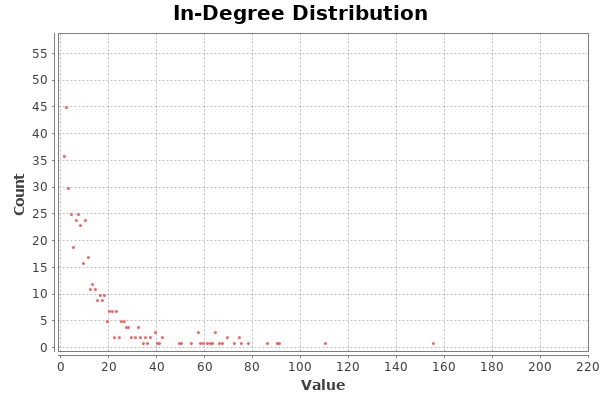
\includegraphics[width=0.5\textwidth]{degree-report/indegree-distribution}
            \label{din}
        }
        \subfigure[Distribución del grado de salida]{
            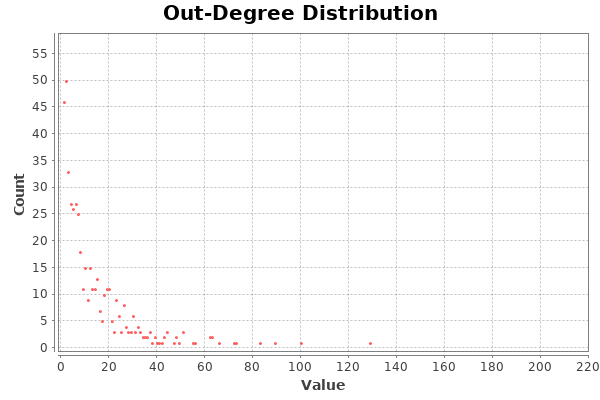
\includegraphics[width=0.5\textwidth]{degree-report/outdegree-distribution}
            \label{dout}
        }
    }
    \caption{Gráficos de distribución del grado de entrada y salida}
    \label{degree}
\end{figure}

El \textbf{diámetro} ($d_{max} = 11$) nos indica cómo de lejos están los nodos más lejanos de la red entre sí. Teniendo en cuenta la gran diversidad de usuarios que sigo, debe de haber bastante relación dentro de las distintas comunidades y además, algunos \textit{hubs} para conectarlas entre sí. Por otro lado, la \textbf{distancia media} ($<d> = 3.5$) representa la eficiencia del flujo de información en la red. En este caso, para que un \textit{Tweet} cualquiera llegase a un usuario, tendría que ser retuiteado unas 3/4 veces. La distancia media en la red aleatoria ($<d_{aleatoria}> = 1.75$) es mucho menor, esto se debe a que en redes aleatorias, la distancia media depende del $log \; N$ lo que implica que $<d>$ sea varios órdenes de magnitud menores que el tamaño de la red. En la \hyperref[dist]{Figura \ref*{dist}} vemos el gráfico de distribución de distancias, en el eje $x$ están representadas las distintas distancias (desde 0 hasta $d_{max}$) y en el eje $y$, el número de caminos en el grafo con esa distancia ($p_d$). Este número de caminos desciende en distancias superiores a $<d>$, lo que nos indica que no existen distancias grandes. Esto es consecuencia de la \textbf{propiedad de mundos pequeños}.

\begin{figure}[!h]
    \centering
    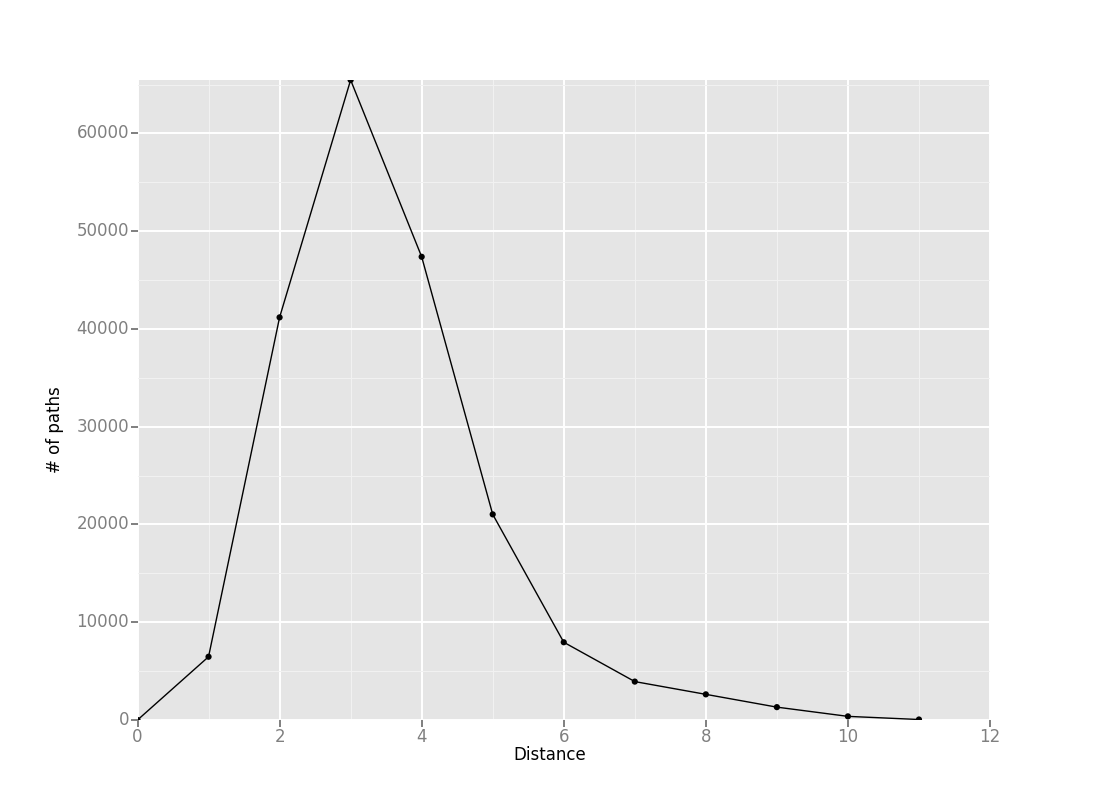
\includegraphics[width=0.7\textwidth]{dist_hist}
    \caption{Distribución de distancias}
    \label{dist}
\end{figure}

En cuanto a la conectividad de la red, vemos que presenta 60 componentes conexas. La componente gigante agrupa el $88.93\%$ de los nodos. La mayoría de componentes conexas están formadas por los nodos con grado 0 que mencioné anteriormente: mirando la \hyperref[degree]{Figura \ref*{degree}}, vemos que hay unos 50 nodos aproximadamente con grado salida 0 y unos 45 nodos con grado de entrada 0. Las otras 10 componentes conexas son las distintas comunidades que hay entre mis amigos. El \textbf{coeficiente medio de clústering} ($<C> = 0.264$) de la red es bastante alto, lo que nos indica un alto grado de clustering local. Esto nos confirma lo que pensé en un principio sobre la transitividad de la red. En la \hyperref[clust]{Figura \ref*{clust}} vemos la distribución del coeficiente de clústering en comparación con el grado ($d_{in}+d_{out}$). Como vemos, el valor del coeficiente de clústering es mucho mayor en los nodos pocos conectados que en los hubs, es decir, los nodos con grado bajo se sitúan en vecindarios muy interconectados y viceversa. Esto es consecuencia de la \textbf{jerarquía de redes}. En comparación con el \textit{coeficiente medio de clústering} de la red aleatoria equivalente, vemos que el de ésta es mucho mayor ($<C_{aleatoria}> = 1.726$), esto se debe a que en redes reales el coeficiente de clústering de un nodo decrece con los grados de los nodos y, además, es independiente del tamaño de la red.

\begin{figure}[!h]
    \centering
    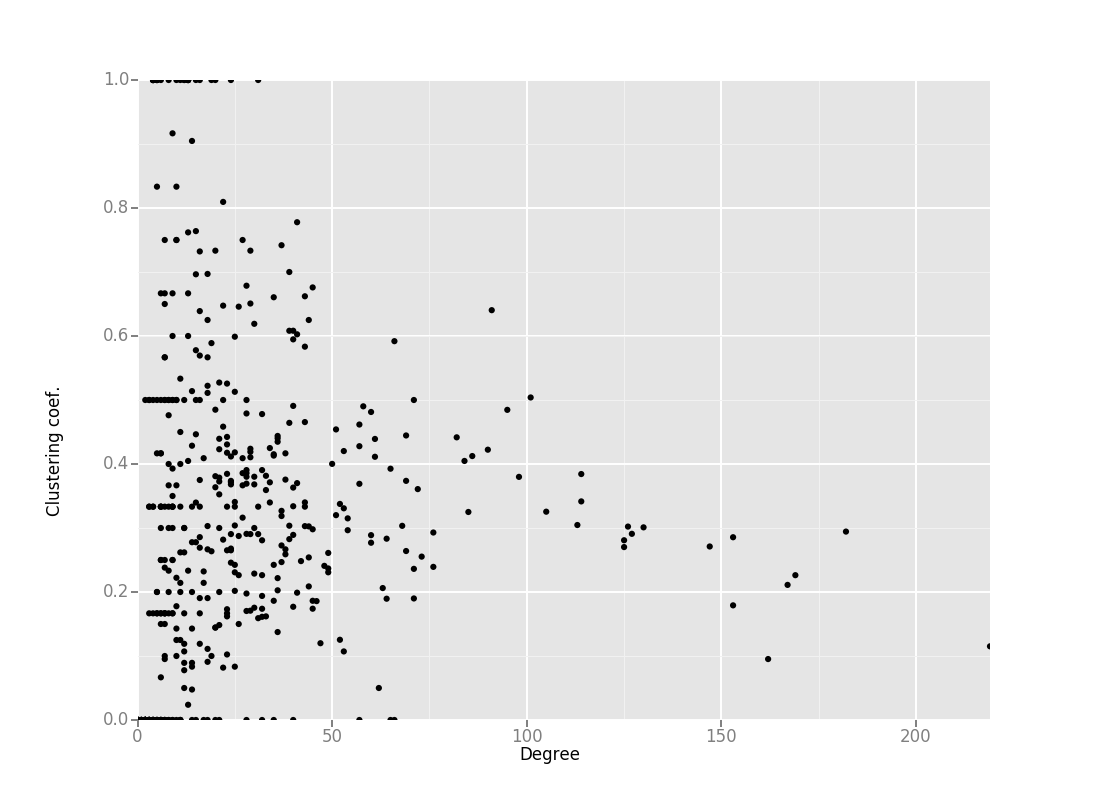
\includegraphics[width=0.7\textwidth]{clust_hist}
    \caption{Distribución del coeficiente de clústering}
    \label{clust}
\end{figure}

El valor de la \textbf{densidad} ($D = 0.022$) es algo bajo, esto nos indica que la conectividad a nivel global de la red es baja. Tiene sentido, ya que dijimos que la red era dispersa ($L \ll L_{max}$).

\section{Cálculo de las medidas de análisis en redes sociales}

\subsection{Influencia}
Como vimos al estudiar la distribución tanto del grado de entrada como el de salida (\hyperref[degree]{Figura \ref*{degree}}) había nodos con un grado muy alto y nodos con grado 0. El grado mide la influencia de un nodo a nivel local, es decir, que no nos daría información sobre un nodo importante a nivel global en la red. En la \hyperref[influencia]{Figura \ref*{influencia}} vemos una representación gráfica de cada nodo en la red. Hay varios nodos de color rojo, que parecen tener mucha influencia. Sin embargo, en la \hyperref[infllocal]{Figura \ref*{infllocal}} vemos la influencia de dos nodos que tienen un alto grado de entrada. El usuario \textit{mfgranaina} (\hyperref[mf]{\thesection .\ref*{mf}}) sólo llega a varios usuarios de Granada, y no a todos ellos, sólo un $13.1\%$ de los nodos de la red. El usuario \textit{jjmerelo} (\hyperref[jj]{\thesection .\ref*{jj}}) sólo llega a usuarios de la OSL y algunos de la ETSIIT, que aunque ésto suponga un $20.11\%$ de la red sigue siendo una influencia a nivel muy local.

\begin{figure}[!h]
    \centering
    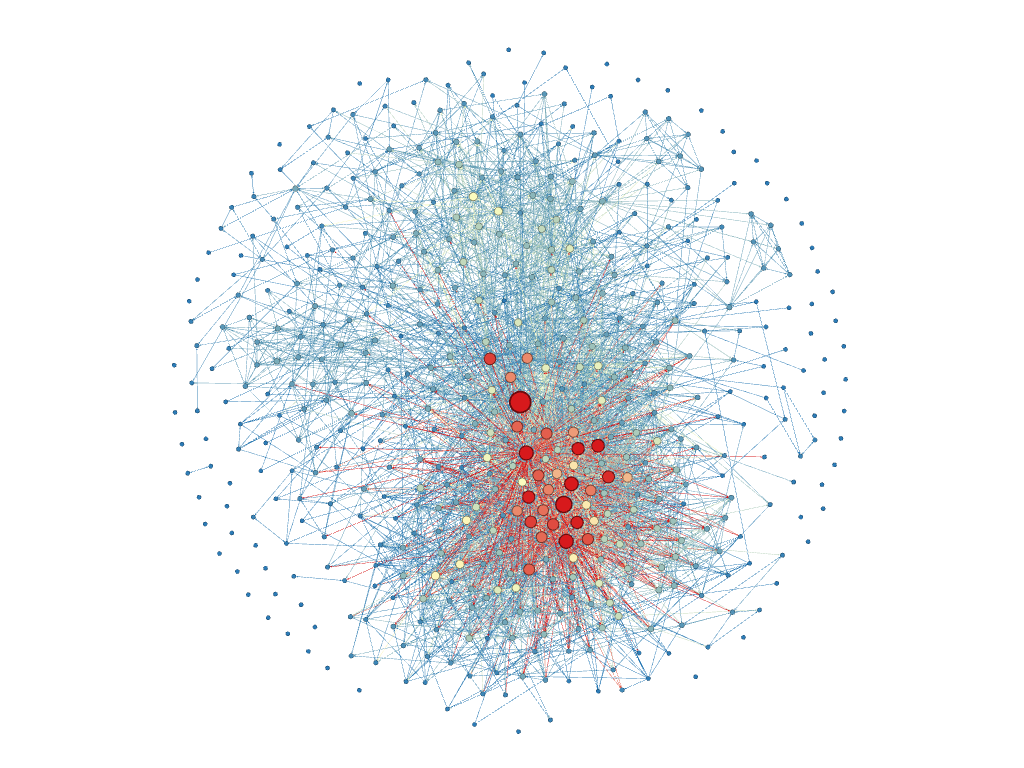
\includegraphics[width=0.7\textwidth]{medidas_locales/influencia}
    \caption{Visualización de la red donde tanto el tamaño de los nodos como el coloreado corresponde con el grado de entrada: a mayor tamaño y un color más calido, más influencia tiene dicho nodo.}
    \label{influencia}
\end{figure}


\begin{figure}[!h]
    \centering
    \mbox{
        \subfigure[Influencia del usuario \textit{mfgranaina}]{
            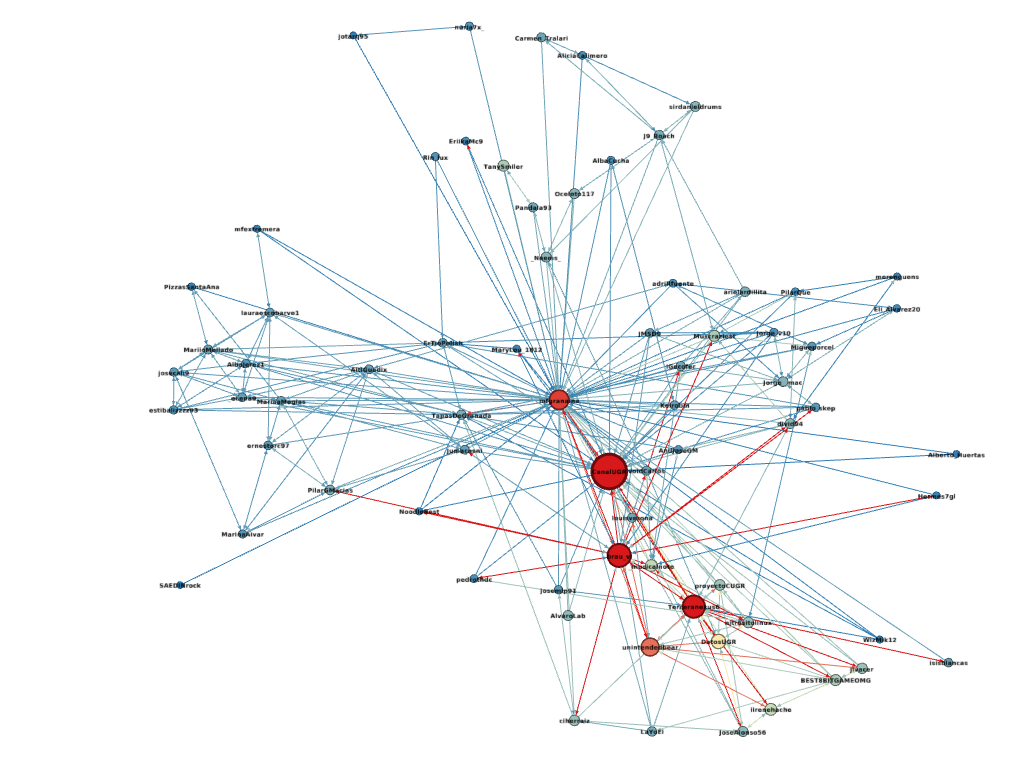
\includegraphics[width=0.5\textwidth]{medidas_locales/influenciamf}
            \label{mf}
        }
        \subfigure[Influencia del usuario \textit{jjmerelo}]{
            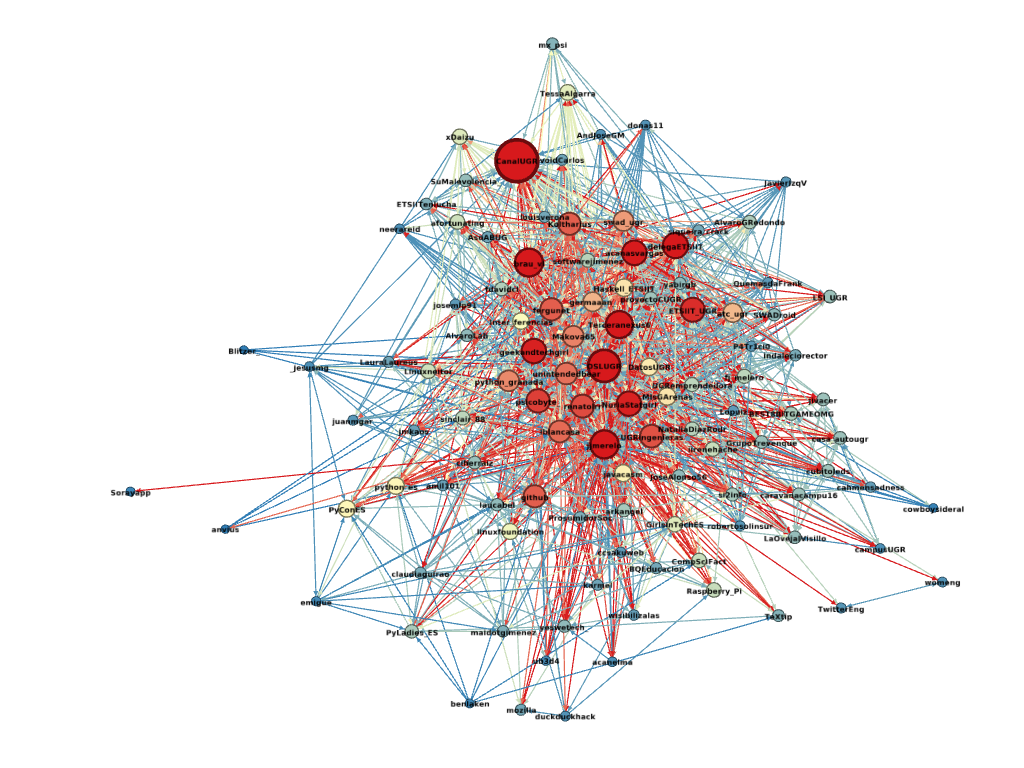
\includegraphics[width=0.5\textwidth]{medidas_locales/influenciajj}
            \label{jj}
        }
    }
    \caption{Influencia de dos nodos con un grado de entrada alto}
    \label{infllocal}
\end{figure}

\subsection{Intermediación}
Con la intermediación, podemos descubrir qué usuario es el que une varias comunidades de la red entre sí. Nos podría interesar para descubrir cómo llegar a varias comunidades a la vez en vez de quedarnos con la perspectiva local del grado. En la \hyperref[intermediacion]{Figura \ref*{intermediacion}} vemos la representación de la intermediación y el grado de entrada en la red. Es importante destacar cómo mucho de los nodos que antes tenían un color muy rojo debido a su alto grado de entrada, tienen ahora un color más bien frío. Esto demuestra esa perspectiva local de la que antes hemos hablado. En la \hyperref[intermediacionbrau]{Figura \ref*{intermediacionbrau}} vemos representada la influencia del usuario \textit{brau\_vl}. Este usuario sólo tiene influencia directa en el $24.91\%$ de la red, pero su influencia llega a muchas comunidades distintas. En parte es normal, ya que Braulio y yo tenemos muchos amigos en común, estudiamos juntos y solemos intercambiar cuentas interesantes para seguir. Por tanto, es normal que después de mí, sea el usuario que está en más comunidades a la vez en mi red.

\begin{figure}[!h]
    \centering
    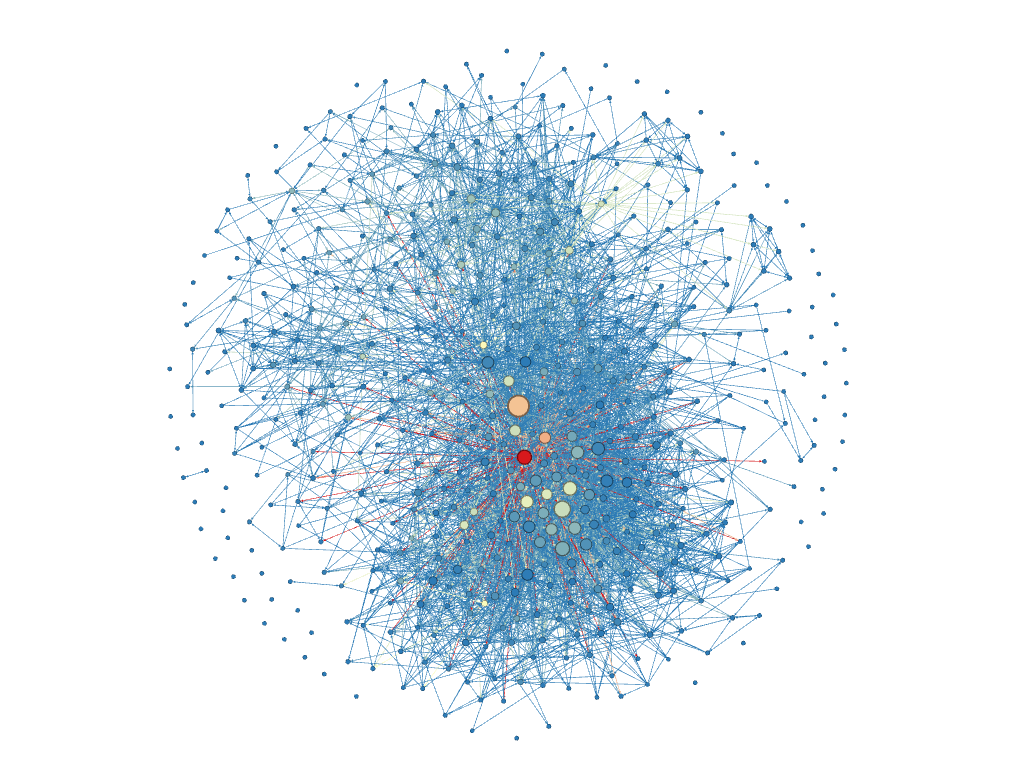
\includegraphics[width=0.7\textwidth]{medidas_locales/intermediacion}
    \caption{Visualización de la red donde tanto el tamaño de los nodos corresponde con el grado de entrada y el coloreado a su intermediación, cuanto más calido sea el color, más intermediación tiene un nodo.}
    \label{intermediacion}
\end{figure}

\begin{figure}[!h]
    \centering
    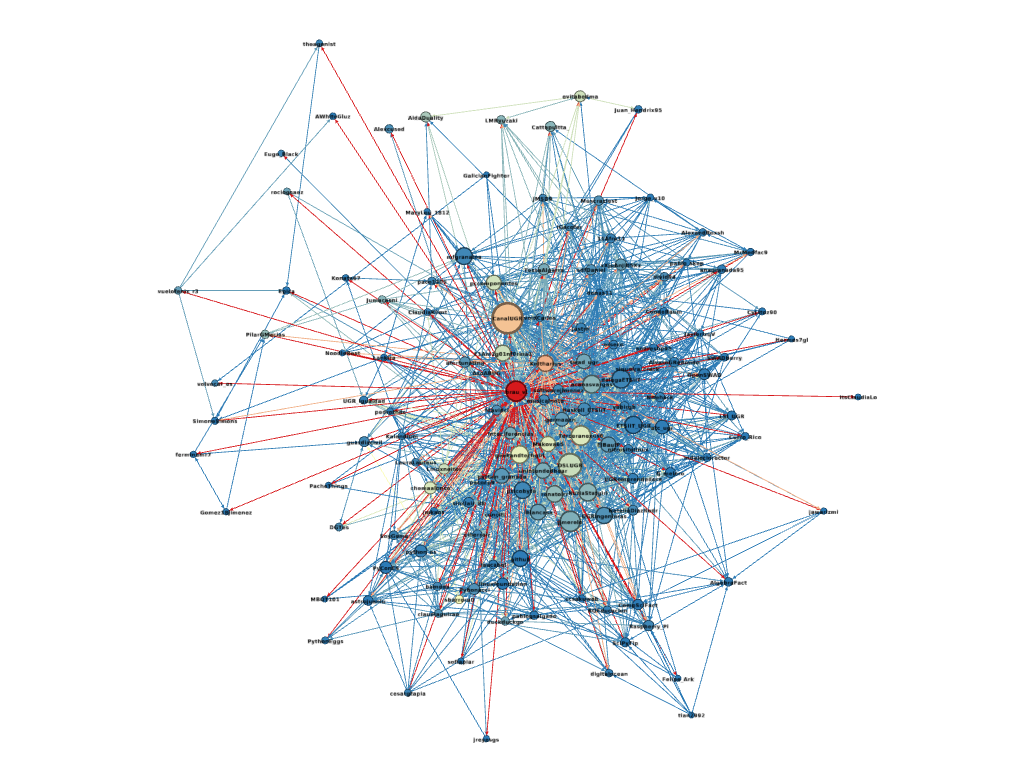
\includegraphics[width=0.7\textwidth]{medidas_locales/intermediacionbrau}
    \caption{Alcance del usuario \textit{brau\_vl}}
    \label{intermediacionbrau}
\end{figure}

A parte de Braulio, no hay ningún otro usuario con un nivel de intermediación alto. Esto se ve también en la \hyperref[bet]{Figura \ref*{bet}} donde tenemos representada la distribución de la intermediación en la red. El valor de la intermediación es muy bajo prácticamente en todos los nodos de la red. De hecho, hay varios nodos con intermediación 0.

\begin{figure}[!h]
    \centering
    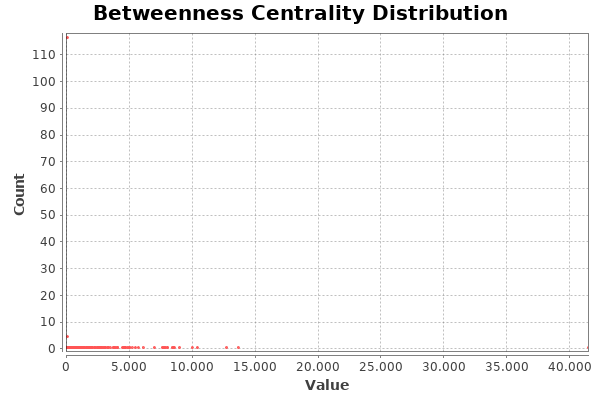
\includegraphics[width=0.7\textwidth]{distance-report/Betweenness-Centrality-Distribution}
    \caption{Gráfico de distribución de la intermediación}
    \label{bet}
\end{figure}

\subsection{Excentricidad}
En la \hyperref[excentricidad]{Figura \ref*{excentricidad}} vemos la representación visual de la excentricidad. Esta medida nos ayuda a ver cuáles son los nodos centrales de la red y cuáles son los periféricos. En este caso, los nodos periféricos son aquellos que sólo sigo yo (y por tanto no están conectados con nadie) o aquellas comunidades aisladas que no tienen apenas conexión con ningún nodo exterior. Los nodos más centrales de la red, no son ni los de mayor grado ni los de mayor intermediación sino que son nodos que debido a su posición, tienen las distancias más cortas en la red. 

\begin{figure}[!h]
    \centering
    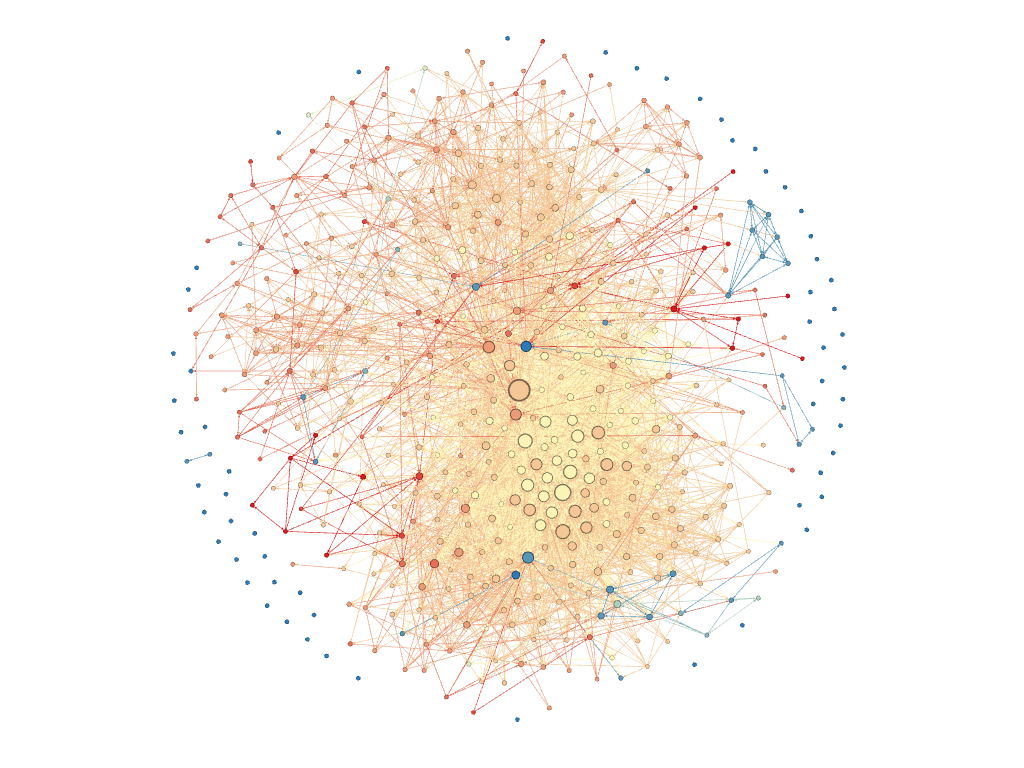
\includegraphics[width=0.7\textwidth]{medidas_locales/excentricidad}
    \caption{Visualización de la red donde tanto el tamaño de los nodos corresponde con el grado de entrada y el coloreado a su excentricidad, cuanto más calido sea el color, más excentricidad tiene un nodo.}
    \label{excentricidad}
\end{figure}

En la \hyperref[excenlocal]{Figura \ref*{excenlocal}} vemos el alcance de dos nodos con un valor alto de excentricidad. Ambos tienen una influencia muy baja en la red, pero están unidos a nodos muy diferentes entre sí, con lo cual consiguen unas distancias muy cortas a todas las distintas comunidades de la red. Esto hace que, desde el punto de vista de la excentricidad, tengan una posición muy central. En las figuras \hyperref[gc]{\thesection .\ref*{gc}} y \hyperref[em]{\thesection .\ref*{em}} vemos el alcance de dos nodos con bastante excentricidad con sólo un nivel de profundidad y en las figuras \hyperref[gc]{\thesection .\ref*{gc2}} y \hyperref[em]{\thesection .\ref*{em2}} vemos el alcance de los mismos nodos pero con un nivel de profundidad más. Al aumentar el nivel, el alcance de ambos nodos se multiplica por 10, esto se debe a las distancias tan cortas que tienen. En el caso de un nodo con un grado muy alto como \textit{jjmerelo}, vimos en la \hyperref[jj]{Figura \thesection .\ref*{jj}} que tenía un alcance al $20.11\%$ de la red, si incrementamos el nivel de profundidad, alcanzaría el $61.25\%$ de la red. Es un valor bastante alto, pero en comparación con el primero, sólo se ha multiplicado por 3. Por tanto, no es un caso tan extremo como el de \textit{guardiacivil} o \textit{efe\_material}.

\begin{figure}[!h]
    \centering
    \mbox{
        \subfigure[Alcance del usuario \textit{guardiacivil} con profundidad 1 ($4.98\%$ de la red)]{
            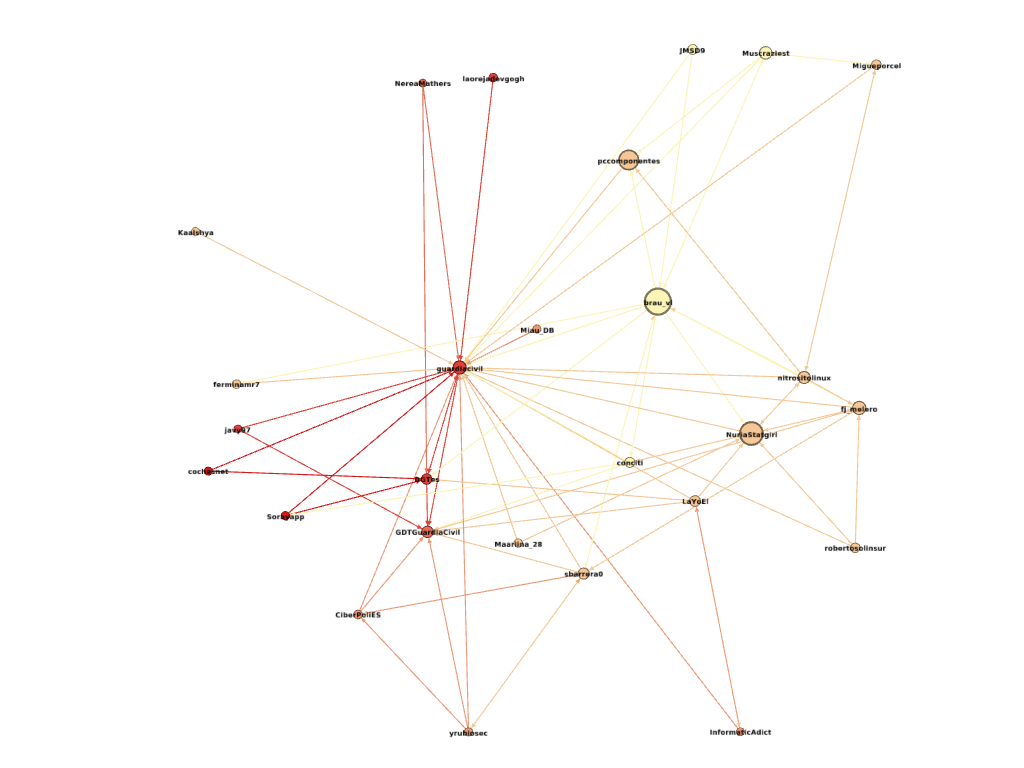
\includegraphics[width=0.5\textwidth]{medidas_locales/excentricidadgc}
            \label{gc}
        }
        \subfigure[Alcance del usuario \textit{efe\_material} con profundidad 1 ($3.51\%$ de la red)]{
            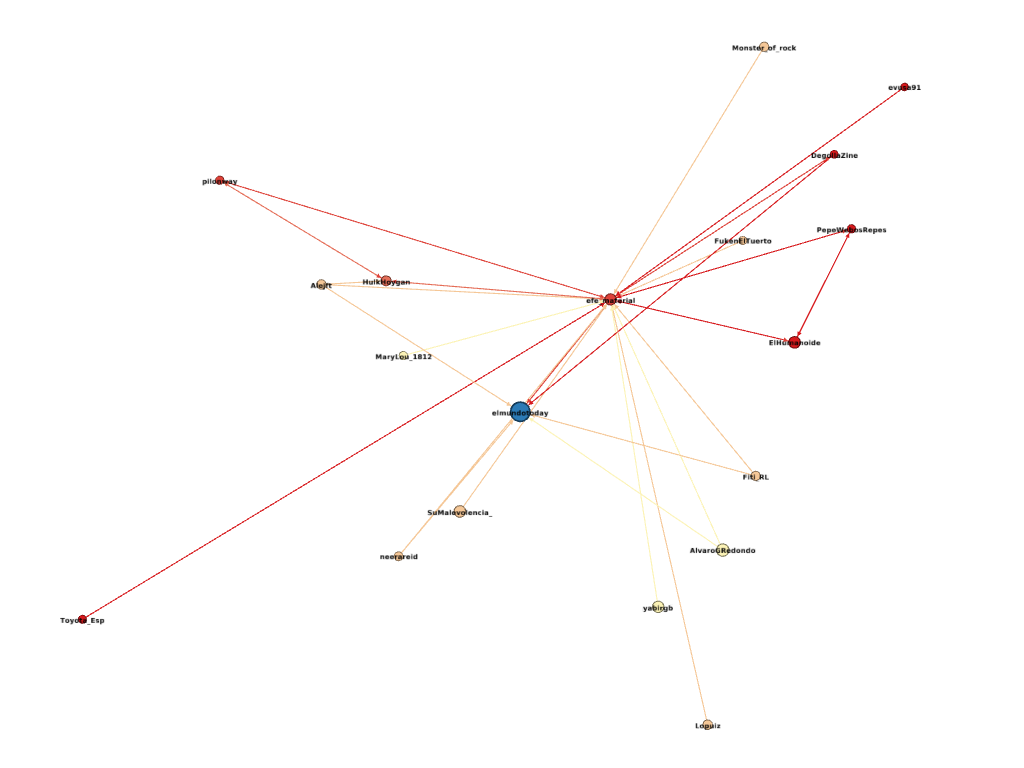
\includegraphics[width=0.5\textwidth]{medidas_locales/excentricidadem}
            \label{em}
        }
    }
    \mbox{
        \subfigure[Alcance del usuario \textit{guardiacivil} con profundidad 2 ($45.57\%$ de la red)]{
            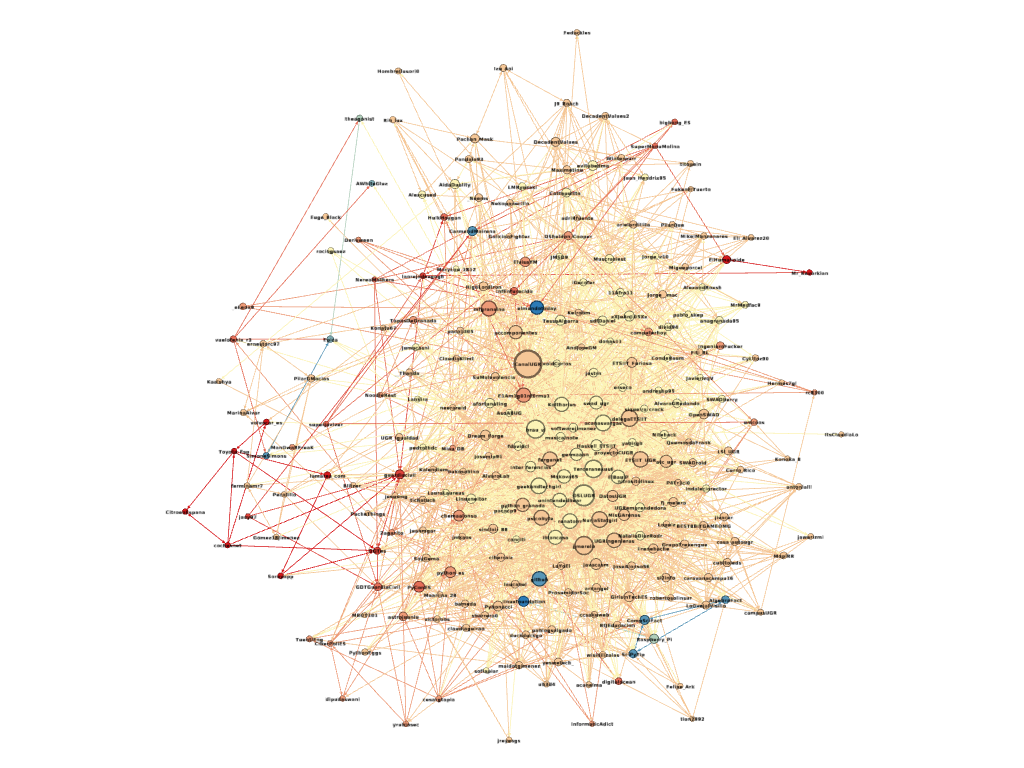
\includegraphics[width=0.5\textwidth]{medidas_locales/excentricidadgc2}
            \label{gc2}
        }
        \subfigure[Alcance del usuario \textit{efe\_material} con profundidad 2 ($34.69\%$ de la red)]{
            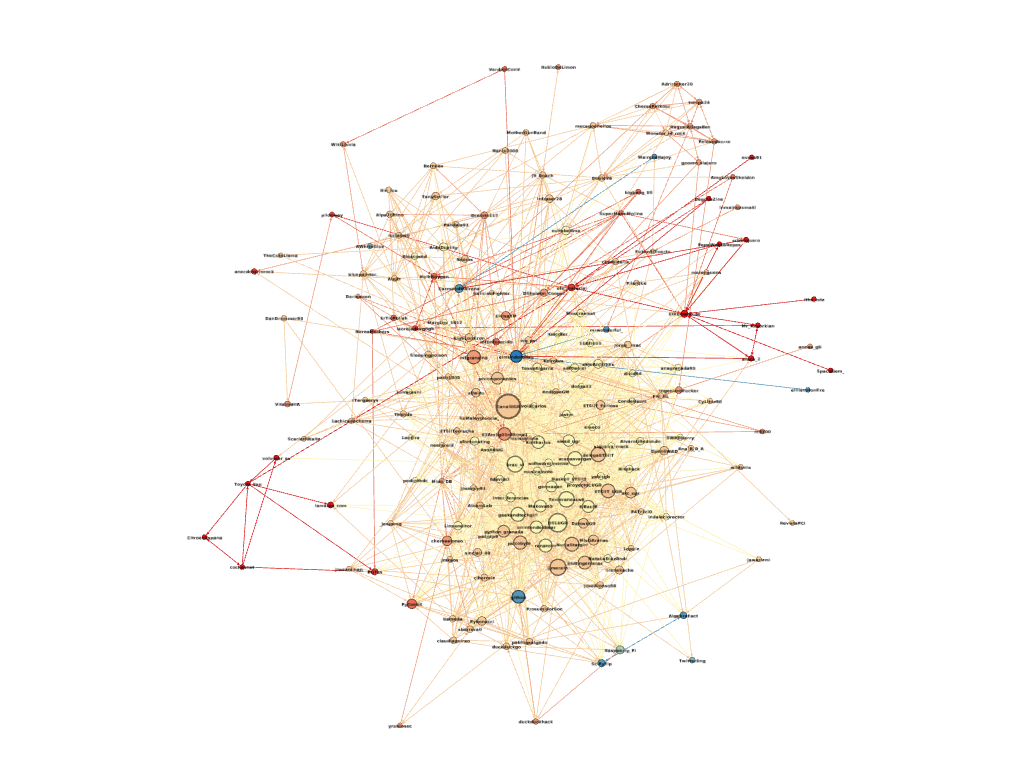
\includegraphics[width=0.5\textwidth]{medidas_locales/excentricidadem2}
            \label{em2}
        }
    }
    \caption{Alcance de dos nodos con una alta excentricidad en la red con dos niveles de profundidad.}
    \label{excenlocal}
\end{figure}

\subsection{Centralidad de vector propio}
En la \hyperref[evv]{Figura \ref*{evv}} vemos una representación visual de la centralidad de vector propio en la red. Esta representación es muy similar a la de la influencia (\hyperref[influencia]{Figura \ref*{influencia}}), aunque hemos eliminado algunos nodos que con su grado de entrada habíamos considerado importantes. El nodo más importante de la red según esta medida es el usuario \textit{CanalUGR}, ya que conecta a toda la comunidad universitaria de mi red. La \textit{OSLUGR} y \textit{jjmerelo} tienen también un valor muy alto de centralidad, en parte debido a que están conectados con la Universidad de Granada y a la gran cantidad de seguidores que tienen. Estos tres usuarios son los que tienen un mayor grado de entrada y, por tanto, también fueron nodos muy importantes al analizar la influencia en la red. Sin embargo, usuarios como \textit{mfgranaina} han pasado a tener una centralidad de vector propio muy pequeña, debido a que, a pesar de tener muchos seguidores ninguno era especialmente importante.

\begin{figure}[!h]
    \centering
    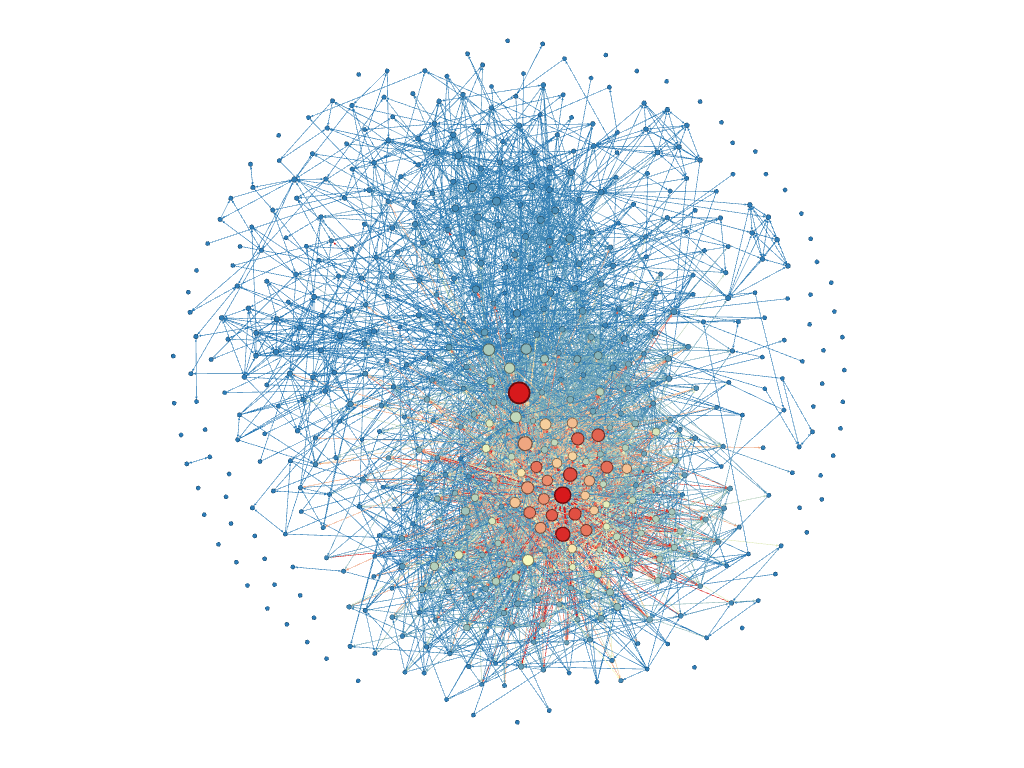
\includegraphics[width=0.7\textwidth]{medidas_locales/eigenvector}
    \caption{Visualización de la red donde tanto el tamaño de los nodos corresponde con el grado de entrada y el coloreado a su centralidad de vector propio, cuanto más calido sea el color, más centralidad de vector propio tiene un nodo.}
    \label{evv}
\end{figure}

\section{Detección de comunidades}
Hemos ido viendo en las secciones previas cómo había indicios de que en esta red hubiese distintas comunidades, debido a la \textit{transitividad}. Vamos a indigar ahora sobre dichas comunidades usando los siguientes algoritmos:

\begin{enumerate}[$\bullet$]
    \item \textbf{Lovaina}: algoritmo greedy que trata de optimizar la modularidad en dos pasos. En primer lugar busca comunidades pequeñas, una vez las encuentra crea una nueva red agregando las comunidades y vuelve a repetir el paso anterior hasta que la modularidad deje de mejorar.
    \item \textbf{Stochastic block model (\textit{degree corrected})}: modelo para generar grafos aleatorios que contengan comunidades. Este algoritmo toma una partición de los nodos en $b$ comunidades, una matriz $B \times B$ de probabilidad de enlaces entre comunidades y una secuencia $k$ de grados de los nodos. Con estos parámetros, trata coloca enlaces de forma aleatoria. El algoritmo usado usa esta idea para encontrar probabilidades de forma probabilística, es decir, que no da la partición óptima sino una buena partición.
    \item \textbf{Nested stochastic block model (\textit{degree corrected})}: capaz de encontrar grupos pequeños en redes grandes y dar una jerarquía multinivel de la red. 
\end{enumerate}

En general, los tres algoritmos han dado resultados muy parecidos, sobre todo a la hora de detectar las comunidades más grandes.

\subsection{Lovaina}
Este algoritmo ha sido ejecutado con \textit{Gephi}. En la \hyperref[lovaina]{Figura \ref*{lovaina}} vemos una visualización de las distintas comunidades que ha encontrado en la red. En la \hyperref[comsl]{Tabla \ref*{comsl}} vemos la proporción de nodos en cada una. Las comunidades más grandes que ha encontrado se corresponden con distintas comunidades que sigo como la oficina del software libre, amigos de la facultad, amigos de mi pueblo, amigos de otros pueblos y gente relacionada con la informática de fuera de Granada. Algunas de las cuentas con un valor alto de excentricidad, que no forman parte de ninguna comunidad, han sido metidas en alguna de estas comunidades, aunque es algo normal. Creo que el punto débil de este algoritmo son las comunidades pequeñas, ya que se ha agrupado en una misma comunidad a mis amigos de murcia y a los personajes de \textit{Big Bang Theory}. Por último, todos los nodos aislados forman una comunidad con un único nodo. Por tanto, creo que la división en comunidades realizada por el algoritmo ha sido bastante acertada, sobre todo en comunidades grandes. 

\begin{figure}[!h]
    \centering
    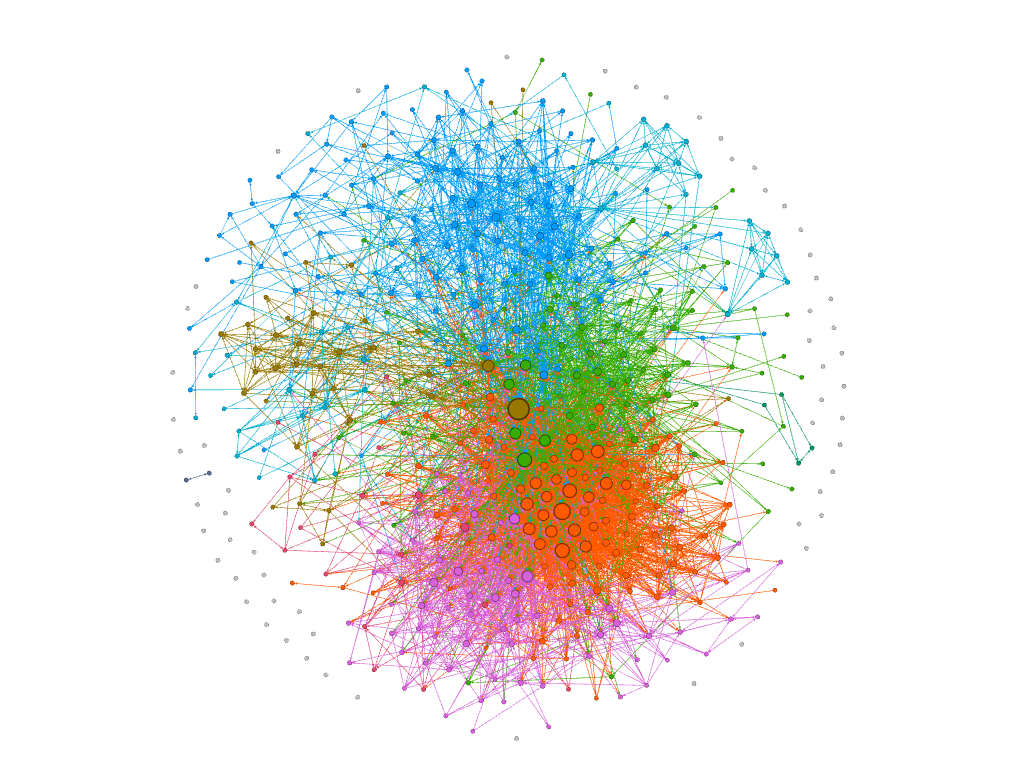
\includegraphics[width=0.7\textwidth]{lovaina}
    \caption{Distribución en comunidades calculada por el método de Lovaina}
    \label{lovaina}
\end{figure}

\begin{table}[!h]
\centering
\begin{tabular}{c | c}
Clase & Proporción de nodos \\
\hline
Azul & $22.69\%$ \\
Naranja & $19.74\%$ \\
Verde & $14.76\%$ \\
Morado & $12.36\%$ \\
Celeste & $8.12\%$ \\
Marrón & $6.83\%$ \\
Magenta & $3.69\%$ \\
Turquesa & $0.74\%$ \\
Marino & $0.37\%$ \\
Gris & $0.18\%$
\end{tabular}
\caption{Comunidades encontradas y su proporción de nodos de la red}
\label{comsl}
\end{table}

\subsection{Stochastic block model}
Este algoritmo ha sido calculado con el paquete de \texttt{python} \textit{Graph tool} \cite{peixoto_graph-tool_2014}. En la \hyperref[blockmodel]{Figura \ref*{blockmodel}} vemos una visualización de las comunidades encontradas en este modelo y en la \hyperref[comsb]{Tabla \ref*{comsb}}, vemos la proporción de nodos en cada clase. En este caso, se han obtenido más comunidades que con el método de Lovaina con un menor tamaño, esto corrige el error que comentábamos anteriormente. Observando las comunidades creadas por el algoritmo, algunas de las comunidades (como la comunidad de la facultad) se han dividido en unas más pequeñas aunque más densas y, además en vez de considerar los nodos aislados comunidades aisladas, los ha considerado todos una misma comunidad.

\begin{figure}[!h]
    \centering
    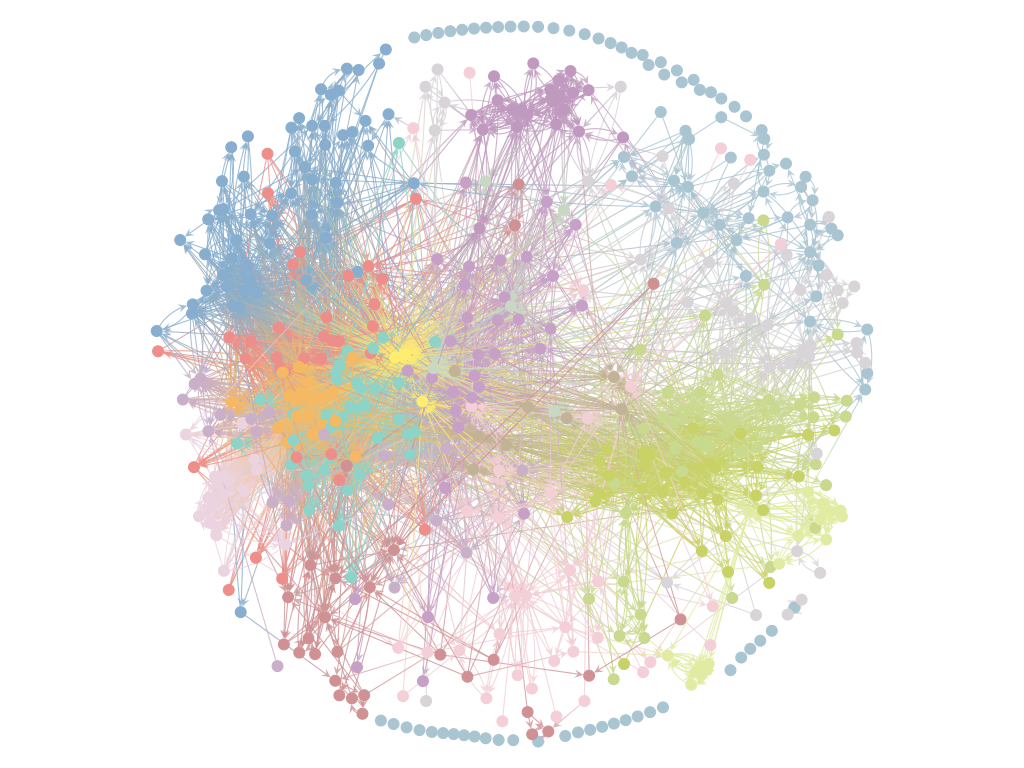
\includegraphics[width=0.7\textwidth]{blockmodel}
    \caption{Distribución en comunidades calculada por el método de Stochastic block model}
    \label{blockmodel}
\end{figure}

\begin{table}[!h]
    \centering
    \begin{tabular}{c | c}
    Clase & Proporción de nodos \\
    \hline
    1  &   $17.343173\%$ \\
    5  &   $10.332103\%$ \\
    9  &    $7.564576\%$ \\
    12  &   $7.380074\%$ \\
    10  &   $6.826568\%$ \\
    0  &    $6.642066\%$ \\
    13  &   $6.273063\%$ \\
    8  &    $5.904059\%$ \\
    3  &    $5.904059\%$ \\
    4  &    $5.166052\%$ \\
    7  &    $3.874539\%$ \\
    14  &   $3.874539\%$ \\
    2  &    $3.690037\%$ \\
    11  &   $3.136531\%$ \\
    15  &   $3.136531\%$ \\
    6  &    $1.476015\%$ \\
    16  &   $0.922509\%$ \\
    17  &   $0.553506\%$ 
    \end{tabular}
    \caption{Comunidades encontradas y su proporción de nodos en la red}
    \label{comsb}
\end{table}

\subsection{Nested stochastic block model}
Este algoritmo ha sido calculado con el paquete de \texttt{python} \textit{Graph tool} \cite{peixoto_graph-tool_2014}. En la \hyperref[nested]{Figura \ref*{nested}} vemos una visualización de las comunidades encontradas en este modelo y en la \hyperref[comsb]{Tabla \ref*{comsn}}, vemos la proporción de nodos en cada clase. Este ha sido el algoritmo que más comunidades ha encontrado. También las comunidades más pequeñas, ya que la primera supone un $19.74\%$ de los nodos y, la segunda sólo un $7.19\%$. Al igual que en el algoritmo anterior, los nodos aislados forman una única comunidad. Los resultados obtenidos son, en general, bastantes parecidos al algoritmo anterior por lo que es difícil escoger entre un resultado u otro.

\begin{figure}[!h]
    \centering
    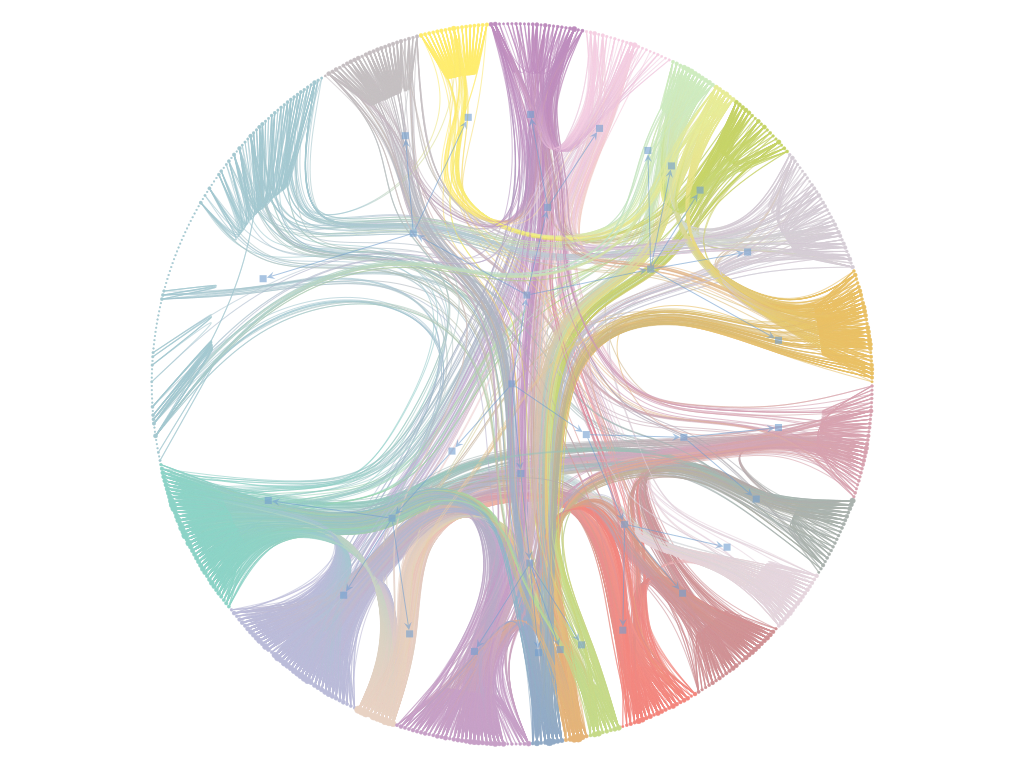
\includegraphics[width=0.7\textwidth]{nested}
    \caption{Distribución en comunidades calculada por el método de Nested stochastic block model}
    \label{nested}
\end{figure}

\begin{table}[!h]
    \centering
    \begin{tabular}{c | c}
    Clase & Proporción de nodos \\
    \hline
    1   &  $19.741697\%$ \\
    0   &   $7.195572\%$ \\
    2   &   $7.195572\%$ \\
    16   &  $6.088561\%$ \\
    15   &  $5.904059\%$ \\
    3   &   $5.166052\%$ \\
    9   &   $5.166052\%$ \\
    5   &   $4.612546\%$ \\
    18   &  $4.612546\%$ \\
    17   &  $4.243542\%$ \\
    13   &  $4.059041\%$ \\
    4   &   $3.690037\%$ \\
    7   &   $3.690037\%$ \\
    10   &  $3.321033\%$ \\
    21   &  $3.136531\%$ \\
    14   &  $2.952030\%$ \\
    19   &  $2.214022\%$ \\
    12   &  $1.845018\%$ \\
    6   &   $1.476015\%$ \\
    11   &  $1.476015\%$ \\
    8   &   $1.107011\%$ \\
    20   &  $1.107011\%$ 
    \end{tabular}
    \caption{Comunidades encontradas y su proporción de nodos en la red}
    \label{comsn}
\end{table}

\newpage
\section{Visualización}
El algoritmo de visualización usado durante todas las visualizaciones mostradas ha sido \textit{Fruchterman \& Reingold}. La razón por la que he escogido esta visualización es debido a que las demás alejaban demasiado a los nodos aislados, provocando una visualización muy pequeña. Con \textit{Fruchterman \& Reingold} se podían apreciar correctamente las distintas comunidades y, además, todos los nodos estaban cercanos entre sí.  En la \hyperref[vis]{Figura \ref*{vis}} vemos varias visualizaciones hechas con distintos algoritmos. En las figuras \hyperref[oo]{\thesection .\ref*{oo}} y \hyperref[yh]{\thesection .\ref*{yh}} vemos los resultados de los algoritmos \textit{OpenOrd} y \textit{Yifan Hu}. Ambos algoritmos alejaban demasiado las componentes aisladas de la red, haciendo que fuese prácticamente imposible obtener una buena visualización de la red completa. Por esta razón, descarté estos dos algoritmos en primera instancia. En las figuras \hyperref[fa]{\thesection .\ref*{fa}} y \hyperref[fa2]{\thesection .\ref*{fa2}} vemos las visualizaciones hechas por los algoritmos \textit{Force Atlas} (\textit{Kamada \& Kawai}) y \textit{Force Atlas 2}. Modificando el parámetro de la gravedad en estas visualizaciones se obtenía un buen resultado de la red, con las componentes aisladas lo suficientemente cerca. Además, nos proporcionan la estructura de metro con la que poder ver los nodos centrales y los más periféricos en la red. Ambas visualizaciones también realizan un buen agrupamiento por comunidades de los nodos, al igual que \textit{Fruchterman \& Reingold}, por lo que hubiesen sido también una buena visualización para este análisis.

\begin{figure}[!h]
    \centering
    \mbox{
        \subfigure[Visualización de la red con el algoritmo \textit{Force Atlas}]{
            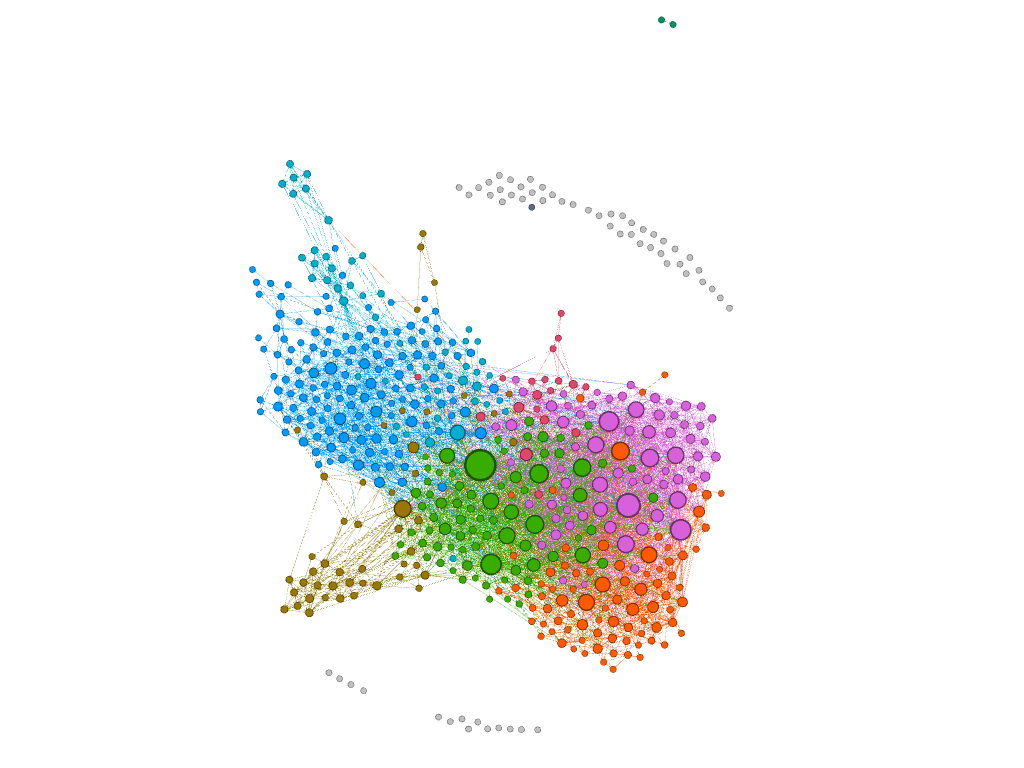
\includegraphics[width=0.5\textwidth]{visualizaciones/forceatlas}
            \label{fa}
        }
        \subfigure[Visualización de la red con el algoritmo \textit{Force Atlas 2}]{
            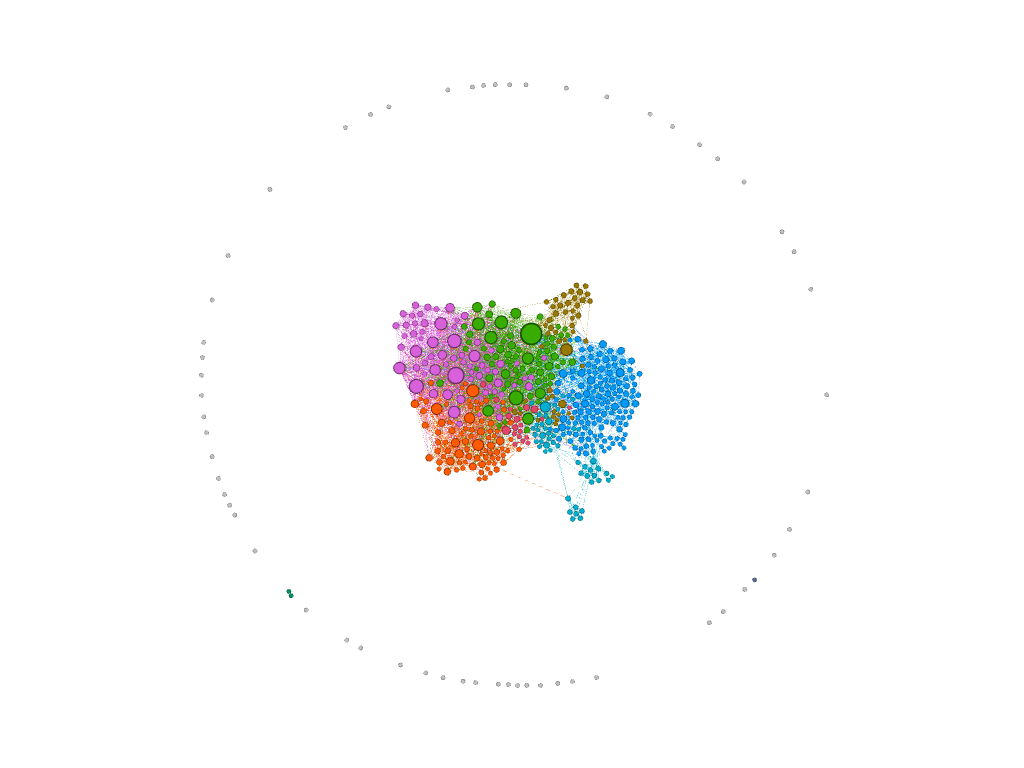
\includegraphics[width=0.5\textwidth]{visualizaciones/forceatlas2}
            \label{fa2}
        }
    }
    \mbox{
        \subfigure[Visualización de la red con el algoritmo OpenOrd]{
            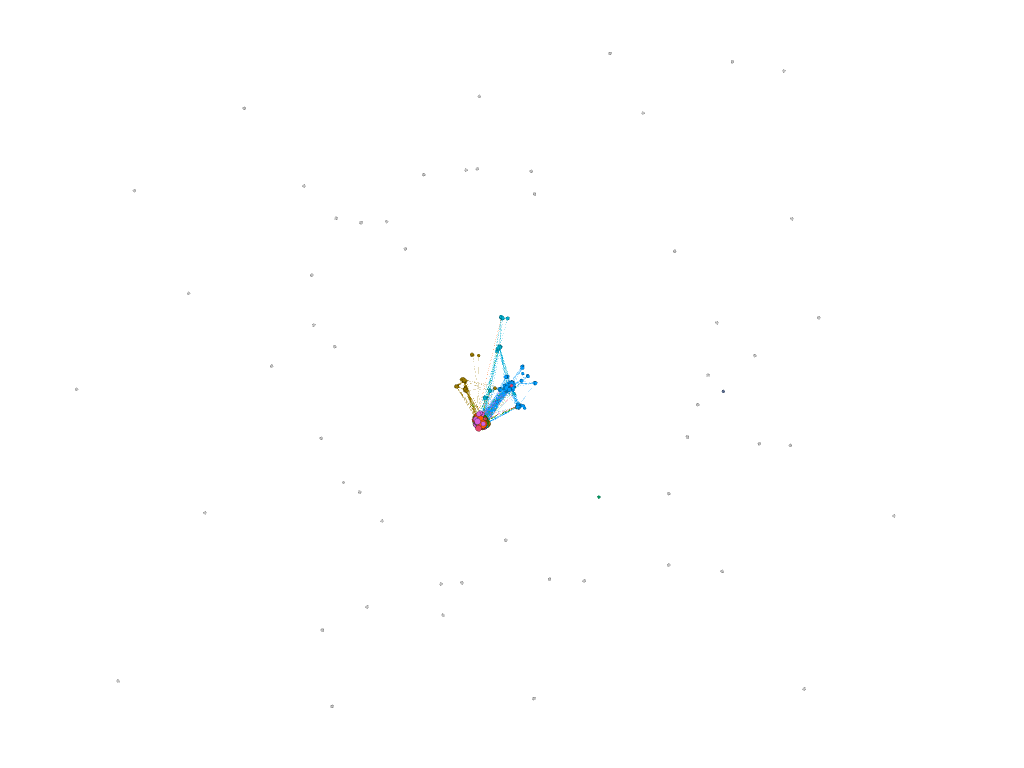
\includegraphics[width=0.5\textwidth]{visualizaciones/openord}
            \label{oo}
        }
        \subfigure[Visualización de la red con el algoritmo Yifan Hu]{
            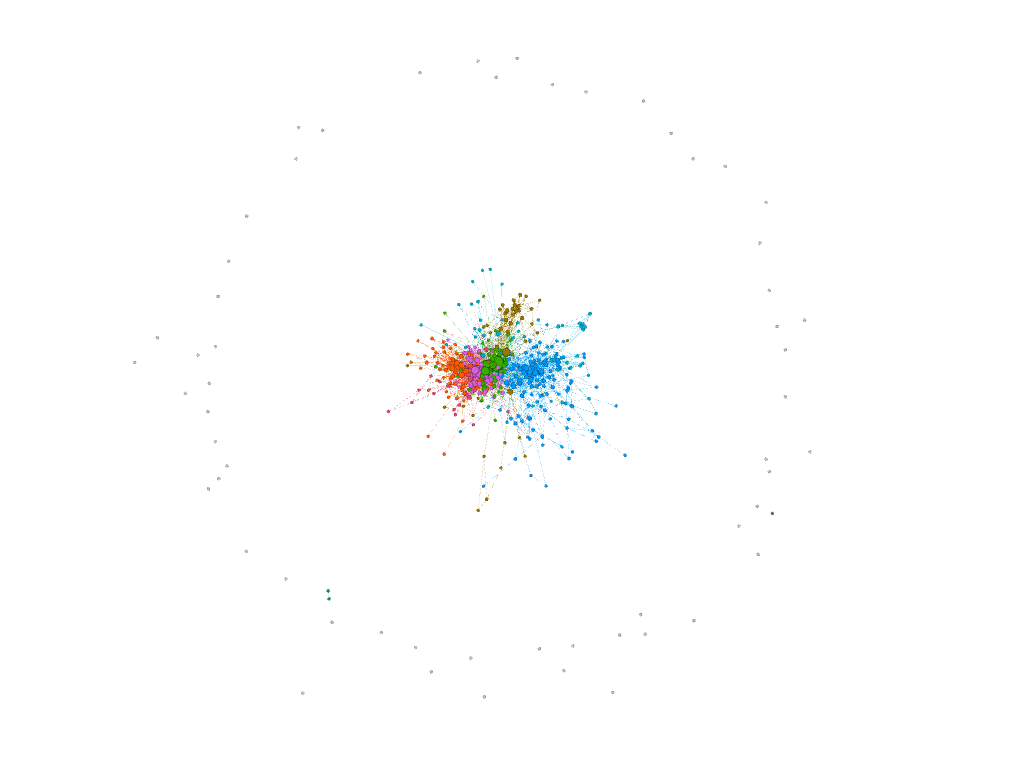
\includegraphics[width=0.5\textwidth]{visualizaciones/yifanhu}
            \label{yh}
        }
    }
    \caption{Visualizaciones de la red con varios algoritmos diferentes}
    \label{vis}
\end{figure}

\section{Discusión de los resultados obtenidos}

Realizando este análisis, he descubierto que los nodos más importantes en mi red están relacionados con la universidad y la facultad, ya que es mi mayor círculo de amigos. Haciendo el análisis de comunidades, he encontrado una buena división para mi lista de amigos, lo que podría facilitarme hacer una división en listas automáticamente con un script (\textit{Tweepy}). Por tanto, creo que he respondido a la pregunta inicial del estudio exitosamente, ya que mi objetivo inicial era encontrar la división en comunidades de usuarios similares entre sí. 

En cuanto a las propiedades de la red, mirando la distribución de grados y distancias concluimos que la red era una red libre de escala y de mundos pequeños. Para verificarlo, he calculado el exponente de la red siguiendo la siguiente ecuación:

\begin{displaymath}
p_k \approx k^{- \gamma} \qquad \longrightarrow \qquad \log p_k \approx - \gamma \log k \qquad \Longrightarrow \qquad \gamma \approx - \frac{\log p_k}{\log k}
\end{displaymath}

Siendo más concreta, he programado un script en el que cuento el número de nodos que tienen un grado $k$, para así obtener $p_k$, repito el proceso tantas veces como vértices haya y hago la media, sin contar los $p_k = 0$ y $k = [0,1]$, ya que $\log 0$ no existe y $\log 1 = 0$, lo cual nos da un fallo al dividir.

Al ser mi red dirigida, he calculado tanto $\gamma^{in}$ como $\gamma^{out}$:

\begin{displaymath}
    \gamma^{in} = 1.5816 \qquad\ \gamma^{out}:  1.575398
\end{displaymath}

Estamos ante un caso muy especial: $\gamma < 2$. Una red con este exponente es una red en la que el grado del mayor hub crece con más rapidez que la red. Esto es debido a que según la siguiente ecuación, el límite natural de una red libre de escala es

\begin{displaymath}
    k_{max} \approx k_{min} N^{\frac{1}{\gamma - 1}}
\end{displaymath}

es decir, según esta ecuación, cuanto más grande sea una red mayor será el grado de su mayor hub. Ahora bien, si $\gamma < 2$ el exponente $\frac{1}{\gamma - 1}$ es mayor a uno y, por tanto, el grado del mayor hub crece más rápido que el tamaño de la red. Este es un caso bastante raro, ya que sólo puede darse si los hubs tienen auto enlaces o si varios enlaces pueden conectar el mismo par de nodos. En este caso no se da ninguna de las dos, pero en la red hay muy pocos hubs y además, es bastante pequeña. Lo que sí podemos confirmar es que \textbf{no estamos ante una red de mundos pequeños o ultra pequeños}. Toda esta información ha sido consultada en \cite{scalefree}.

\mypy[label={exponente.py}]{../exponente.py}

En comparación con otras redes estudiadas en la asignatura, esta es demasiado pequeña y prácticamente se podría considerar de juguete. Sin embargo, me ha parecido una forma muy creativa de resolver mi problema. Las otras redes libres de escala vistas en el tema 5 de la asignatura, y disponibles también en \cite{scalefree}, son redes de mundos ultra pequeños con $3 < \gamma < 2$. De las estudiadas, creo que la más similar a mi red es la \textit{Actor Network}, ya que tiene un $<k>$ alto y un $\gamma$ de $2.15$, es decir, pequeño aunque no tanto como en mi caso (aunque, como he dicho, creo que en mi caso se debe a que la red es muy pequeña).

\bibliography{bibliografia} %archivo citas.bib que contiene las entradas 
\bibliographystyle{siam} % hay varias formas de citar

\end{document}

